\begin{savequote}[75mm]
   You know nothing, Jon Snow.
\qauthor{Ygritte, A Song of Ice and Fire by George R. R. Martin}
\end{savequote}

\chapter{Wprowadzenie}
\newthought{Skąd wzięły się planety?} Pytanie, które nurtuje ludzkość od
zamierzchłych czasów. Konkretne rozważania teoretyczne dotyczące pochodzenia
planet mają długą historię sięgającą przynajmniej XVIII wieku, kiedy to Immanuel
Kant wysunął ,,Hipotezę mgławicową''~\cite{ImmanuelKant.etal:2008}. Już wtedy
unikalność Układu Słonecznego stanowiła przedmiot debaty. Dopiero na początku XX
wieku pogląd, iż układy planetarne są czymś powszechnym we Wszechświecie, został
zaakceptowany przez środowisko naukowe, a w~roku 1992 została odkryta pierwsza,
pozasłoneczna planeta orbitująca pulsar PSR 1257+12b~\cite{1992Natur.355..145W}.
Dziś znamy ponad 1800 układów planetarnych oribtujących gwiazdy znajdujące się
na różnorakich etapach ewolucji. Pomimo tego bogactwa danych obserwacyjnych
i~wieloletnich badań teoretycznych, odpowiedź na pytanie \emph{skąd wzięły się
planety} pozostaje niejednoznaczna.

%\begin{figure}[!ht]
%\centering
%\includegraphics[width=0.8\textwidth]{figures/laplace.png}
%\caption{Model mgławicy Laplace'a: (a) rotująca mgławica; (b) kolapsująca
%mgławica ulega spłaszczeniu wzdłuż osi rotacji; (c) soczewkowaty kształt
%mgławicy; (d) pierścienie materii pozostawione przez zapadający się obiekt
%centralny; (e) zagęszczenia na poszczególnych pierścieniach kolapsują tworząc
%planety. (Obrazek z~pracy Woolfson, 1993)} 
%\label{fig:laplace}
%\end{figure}

\section{Paradygmat powstawania planet}
\subsection{Narodziny gwiazdy}
Formowanie się planet jest nierozerwalnie związane z~narodzinami gwiazd, które
biorą swój początek w~gęstych pyłowo--gazowych obłokach materii. Zanurzone w
gorącym ośrodku międzygwiazdowym, początkowo w~stanie równowagi termodynamicznej
z otaczającym je gazem, obłoki takie często występują w~ogromnych kompleksach i
obserwowane są jako ciemne mgławice molekularne~\cite{Tielens05}. W~ich pobliżu
odnajdywane są gwiazdy~\emph{T Tauri} -- obiekty zmienne o jasności większej niż
wynikałoby to z~ich temperatur efektywnych, co sugeruje ich młody wiek,
nieprzekraczający 1~\Myr~\cite{H62}. Obserwowane temperatury efektywne sugerują,
iż we wnętrzach nie panują dostatecznie wysokie temperatury, aby mogły zachodzić
już reakcje spalania wodoru~\cite{CK79}. Część obserwowanych gwiazd T~Tauri jest
częściowo zanurzona w~małych, ciemnych i~gęstych obłokach materii. Jak pokazują
obserwacje na falach radiowych i~w~podczerwieni, obłoki te są na tyle gęste, że
siła wynikająca z gradientu ciśnienia jest w~stanie zrównoważyć siłę pochodzącą
od samograwitacji~\cite{WT02}. Ich wewnętrzna struktura jest wysoce
hierarchiczna, tzn. we wnętrzu pojedynczego gęstego obłoku o masach rzędu
tysięcy mas słonecznych rozciągającego się na wiele parseków, znajdują się dużo
gęstsze obiekty o masach rzędu $1\Msun$ i~rozmiarach rzędu $0.1\pc$~\cite{M85,
LSM93}. Obserwacje rotacyjnych linii emisyjnych molekuły NH$_3$ pozwalają
szacować typowe koncentracje gazu w~obłokach na $10^{4}\cm^{-3}$~\cite{BM89}.
Nieregularny brzeg obłoków, w~połączeniu z~ich w~przybliżeniu fraktalną
strukturą, interpretowany jest jako obecność silnej turbulencji w samych
obłokach~\cite{E00, FPW91}. Nie jest jasne czy ta struktura jest przejściowym
etapem ewolucji całego kompleksu obłoków, czy też quasi-stacjonarnym
stanem~\cite{L94}. Zródła turbulencji można upatrywać w supernowych, wiatrach
gwiazdowych, promieniowaniem masywnych gwiazd oraz niestabilnościach związanych
z polem magnetycznym~\cite{NP03, MLK04}. 
Typowe temperatury obłoków molekularnych wynoszą od
10 do 20\K. Za efektywne chłodzenie początkowo odpowiada emisja w~podczerwieni
molekuły CO~\cite{MSWG82}, jednakże w~trakcie kolapsu grawitacyjnego gaz sprzęga
się termicznie z~pyłem, który wypromieniowuje nadwyżkę energii
w~podczerwieni~\cite{HN65, MI00} przez co temperatura całego zapadającego się
obłoku pozostaje stała w czasie.

\par Procesy zachodzące w~samych obłokach tj. turbulencja, samograwitacja, lub
w ośrodku zewnętrznym tj.  wybuchy supernowych mogą powodować wzrost gęstości
poszczególnych zagęszczeń w~obłoku. W~momencie, w~którym obszar gęstej materii
przekroczy  masę krytyczną, nazywaną masą Jeansa $M_J$~\cite{J1902, J1928},
grawitacja przeważa i~chmura zaczyna się zapadać (rysunek 1a). Masa Jeansa
zależy od temperatury kinetycznej ośrodka $T$ oraz jego gęstości
$\rho$~\cite{H64}:
%
\begin{equation} M_J \sim
   \left( \frac{k_B T}{G} \right) ^\frac{3}{2} {\rho}^{-\frac{1}{2}},
\end{equation}
%
gdzie $k_B$ jest stałą Boltzmanna a $G$ jest stałą grawitacji.
Dla wymienionych powyżej typowych warunków panujących wewnątrz obłoków materii
międzygwiazdowej~\cite{BM89}, masa Jeansa przyjmuje wartość:
%
\begin{equation}
 M_J \approx 2.9 M_{\odot} \left(\frac{T}{10\K}\right)^{1.5} 
 \left(\frac{n}{10^4\cm^{-3}}\right)^{-0.5},
\end{equation}
%
gdzie $n = \rho_g / \mu \mH$ jest koncentracją cząstek materii.
Gdyby gradient ciśnienia był niewystarczający do utrzymania równowagi, kolaps
obłoku następowałby w~tzw. skali czasowej spadku swobodnego~\cite{Spitzer1978}:
%
\begin{equation}
   t_{\textrm{ff}} \sim \frac{1}{\sqrt{G\rho}} \sim 10^5\yr
   \left(\frac{n}{10^4\thinspace \cm^{-3}}\right)^{-0.5}.
\end{equation}
%
W~rzeczywistości gradient ciśnienia w~niewielkim tylko stopniu spowalnia
zapadanie się materii~\cite{T82}. Obliczenia numeryczne pokazują, że profil
gęstości materii w~zapadającym się, sferycznie symetrycznym obłoku, pozbawionym
pola magnetycznego i turbulencji, asymptotycznie zbiega do funkcji
proporcjonalnej do $r^{-2}$~\cite{L69}. W~rezultacie tylko niewielka część masy
obłoku formuje protogwiazdę, reszta materii zostaje uwięziona w~formie
rozciągniętej otoczki opadającej na obiekt centralny. Przy braku rotacji
i~zaniedbaniu wpływu pola magnetycznego otoczka opada radialnie w~tempie
proporcjonalnym do $c_s^3 / G$, gdzie $c_s$ jest izotermiczną prędkością
dźwięku.  Stała proporcjonalności wynosi od około jedności~\cite{S77} do
kilkudziesięciu~\cite{H77}.

\par Jak już wcześniej wspomniano, pole magnetyczne odgrywa istotną rolę w
dynamicznej ewolucji całego kompleksu obłoków molekularnych i~należy spodziewać
się obecności silnego pola magnetycznego w~zapadającym się obłoku molekularnym i
jego przeciwdziałania sile samograwitacji~\cite{MC99}. Jednym z możliwych
mechanizmów zapoczątkowujących kondensację materii w~centrum grawitacji jest
dyfuzja ambipolarna, która zachodzi w~skalach czasowych rzędu
$10^7$~lat~\cite{MZGH93}.  Dzięki stopniowemu zwiększaniu masy, centralna część
podtrzymywanego przez pole magnetyczne obłoku ulega powolnej kontrakcji do
momentu osiągnięcia koncentracji materii rzędu $10^{5}\cm^{-3}$, dla której
siła samograwitacji przeważa nad ciśnieniem magnetycznym i~rozpoczyna się
niepohamowany kolaps~\cite{BM94, CB00}. Niedawne eksperymenty
numeryczne~\cite{JHCF13} sugerują, że uwzględnienie wpływu turbulencji podczas
kolapsu pozwala efektywniej przełamać przeciwdziałający samograwitacji wpływ
pola magnetycznego, nawet dla silnie namagnesowanego ośrodka.

\par W powyższych rozważaniach całkowicie zaniedbano wpływ rotacji na ewolucję
formującej się protogwiazdy. Większość obserwowanych obłoków materii z której
formują się potem gwiazdy rotuje~\cite{GBFM93}, co wydaje się być naturalną
konsekwencją turbulencji obecnej w~obłokach~\cite{BB00}. Typowy moment pędu
szacowany w~obłokach protogwiazdowych jest przynajmniej o rząd większy niż
moment pędu, który posiadałaby gwiazda rotując z~maksymalną prędkością
równoważącą siłę samograwitacji. 

Fakt ten implikuje konieczność uwzględnienia mechanizmu odpowiedzialnego za
radialny transport momentu pędu Rotacja powoduje, że materia nie opada
centralnie na centrum grawitacji, lecz formuje dysk podtrzymywany przez
równowagę pomiędzy radialną składową siły grawitacji oraz siłę
odśrodkową~\cite{TSC84}. Biorąc pod uwagę masę opadającą z~otoczki, formujący
się dysk jest marginalnie stabilny, bądź jest całkowicie niestabilny
grawitacyjnie~\cite{SKBT94}. W~rezultacie tworzą się w~nim spiralne fale
gęstości, które pod wpływem momentu siły wynikającego z oddziaływania
grawitacyjnego porcji gazu tworzącego dysk, napędzają akrecję materii na
protogwiazdę~\cite{St00}.
Akrecja materii przebiega w sposób nie zaburzony jeżeli fluktuacje gęstości
wysycają się na odpowiednio niskim poziomie. W przeciwnym razie dysk mozę
rozpaść się tworząc układ podwójny lub wielokrotny.
%Ewolucja masywnego dysku zostanie dokładnie opisana w
%podrozdziale~\ref{sec:GI}. 

\par Formujące się w~centrum zagęszczenie staje się nieprzezroczyste dla
termicznej emisji pyłu przy gęstościach gazu większych niż $10^{-13}\g\cm^{-3}$
$(2\cdot10^{10}$ H$_2\cm^{-3})$~\cite{L69} w~wyniku czego temperatura wnętrza
obłoku zaczyna rosnąć. Kończy to etap izotermicznego kolapsu. Nieprzezroczyste
jądro obłoku staje się adiabatyczne (wykładnik adiabatyczny H$_2$: $\gamma =
7/5$~\cite{L69}) dla gęstości powyżej $10^{-12}\g\cm^{-3}$. W adiabatycznie
ściskanym gazie ciśnienie prowadzi do praktycznie
całkowitego zatrzymania kolapsu dla gęstości centralnej $\sim 2\cdot
10^{-10}\g\cm^{-3}$ w rezultacie gaz  osiąga równowagę hydrostatyczną. Gaz
z~otoczki nie przestaje być jednak akreaowany i gęstość oraz temperatura jądra
cały czas rośnie. Krytycznym momentem jest osiągnięcie przez gaz temperatury
$2000\K$, dla której następuje dysocjacja molekuły H$_2$ i~gwałtowny spadek
wykładnika adiabatycznego poniżej wartości $4/3$. Ta druga faza kolapsu zachodzi
podobnie jak początkowy kolaps izotermiczny. Faza ta trwa, aż do momentu kiedy
wodór zostanie zjonizowany przez wzrost temperatury i~wykładnik adiabatyczny
gazu wzrośnie do wartości $5/3$.  Wzrost ciśnienia prowadzi do uformowania
drugiego jądra pozostającego w równowadze hydrostatycznej. Posiada ono dość
niewielką masę rzędu $10^{-3}\Msun$ i~rozmiar około $1\Rsun$~\cite{MI00}.
Całkowita masa formującej się protogwiazdy nie przekracza na tym etapie
$10^{-2}\Msun$.  Dominującym procesem staje się akrecja materii, która musi
dostarczyć pozostałe 99\% masy do rodzącej się gwiazdy. 

W~trakcie akrecji, protogwiazda cały czas pozostaje niewidoczna dla obserwatora,
ponieważ jest przysłonięta przez pył znajdujący się w~opadającej otoczce.
Klasyfikacja obserwacyjna takiego układu określa obiekty na tym etapie mianem
\emph{klasy zero}~\cite{andre} (rysunek 1b). Ich obserwowana temperatura jest
stosunkowo niska $(T \lesssim 30\K)$. Obiekty te charakteryzują się maksimum
w~rozkładzie energii promieniowania wypadającym w~dalekiej podczerwieni, bez
wykrywalnej nadwyżki w~bliskiej podczerwieni. Z czasem kiedy z~otoczki ubywa
materii, obszar optycznie gruby staje się coraz mniejszy i~maksimum
wypromieniowywanej energii przesuwa się w~kierunku bliższej podczerwieni.
Ostatecznie światło samej gwiazdy przebija się przez pozostałość otoczki, dzięki
czemu można zaobserwować charakterystyczne, dwuskładnikowe widmo (patrz
Rysunek~\ref{fig:sed}). Obserwatorzy wprowadzili prostą klasyfikację tak młodych
obiektów dzieląc je na 4 klasy: 0, I, II i~III, które oznaczają położenie
maksimum w~rozkładzie energii promieniowania odpowiednio na falach:
submilimetrowych, dalekiej podczerwieni, bliskiej podczerwienie i~w~zakresie
widzialnym. Poszczególne klasy odpowiadają też różnym fazom akrecji materiału i
różnią się długością trwania. Protogwiazdy znajdują się w~klasie 0 przez około
kilkadziesiąt tysięcy lat~\cite{FSSK06}. W~tym czasie następuje gwałtowna
akrecja materii.  Klasa I jest o rząd wielkości dłuższa (kilka $10^5$ lat), zaś
maksymalny wiek obserwowanych gwiazd T Tauri (klasa II) wynosi $10^6$
lat~\cite{HCGD98}.  Dla obiektów klasy III w~widmach zanikają wszelkie struktury
przypisywane materii okołogwiazdowej~\footnote{ang. \emph{weak-line T Tauri
stars}}.  Protogwiazda traci materię z~dysku na skutek jego
fotoewaporacji~\cite{ACP06} i~wiatru gwiazdowego~\cite{PN86}. Wiele
obserwowanych gwiazd T Tauri wykazuje w~obserwowanych widmach już tylko
szczątkową akrecję $10^{-7} \div 10^{-8} \Msun\rok^{-1}$~\cite{Hart98}. Tak niski
poziom akrecji nie jest już w~stanie znacząco wpłynąć na masę gwiazdy i~proces
jej formowania można uznać za zakończony.

\subsection{Powstawanie planet}

Proces formowania się planet najprawdopodobniej nie jest pojedynczym procesem,
lecz złożeniem wielu różnych etapów, w~których każdy kolejny krok bazuje na
produktach poprzedniego. Już w~połowie XX wieku Carl von
Weizsacker~\cite*{1943ZA.....22..319W} i~Gerard
Kuiper~\cite*{1951PNAS...37....1K} zapostulowali, iż dynamiczna ewolucja obłoku
protoplanetarnego prowadzi do utworzenia się lokalnych zagęszczeń gazu i~pyłu.
Postulowany model zakłada, że mikroskopijne cząsteczki pyłu sklejają się ze sobą
tworząc coraz to większe ciała --- \emph{planetezymale}. Kiedy planetezymale
osiągną rozmiary $\sim 10\m$ ich wzajemne oddziaływanie grawitacyjne zaczyna
przeważać nad siłami tarcia aerodynamicznego. Następnie planetezymale zaczynają
się zderzać formując obiekty o rozmiarach rzędu tysięcy kilometrów ---
protoplanety. Protoplanety zaś są na tyle masywne, iż są w~stanie akreować
otaczający je gaz. Bardziej szczegółowo można podzielić formowanie się planet na
4 etapy:

\begin{description}
   \item[i) koagulacja ziaren pyłu $\left(\mum \rightarrow \km\right):$] 
      Z doświadczeń laboratoryjnych wynika~\cite{BW08}, że drob\-ne cząsteczki pyłu
      mogą na skutek wzajemnych zderzeń zwiększać swoje rozmiary. ,,Spoiwem'' stają
      się siły van der Waalsa bądź oddziaływanie elektrostatyczne. Opierając się
      na analizie drogi swobodnej jednorodnej frakcji cząstek pyłu o promieniu
      $a$, można określić charakterystyczną skalę czasową koagulacji jako 

   \begin{equation}\label{coag} 
      t_{\textrm{coag}} % = \frac{1}{n_d \sigma \Delta v}
      \sim \frac{a}{\Delta v}\frac{\rho_p}{\rho_d} \approx 
      10^{-12} \rho_d^{-1}\yr\thinspace
      \left(\frac{a}{1\mum}\right)
      \left(\frac{\Delta v}{0.1\m\s^{-1}}\right)^{-1}
      \left(\frac{\rho_p}{3\g\cm^{-3}}\right),
   \end{equation}

   gdzie $\Delta v$ jest średnią prędkością względna cząstek, $\rho_p$ jest
   gęstością materiału budującego cząstki natomiast $\rho_d$ jest gęstością
   ośrodka pyłowego w~dysku.  Biorąc pod uwagę typowe gęstości pyłu w~obłokach
   gwiazdowych $(\rho_d \sim 10^{-20}\g\cm^{-3})$ proces ten zachodzi w~skali
   czasowej milionów lat. Jednakże dla dysków protoplanetarnych o typowych
   gęstościach rzędu $10^{-10}\g\cm^{-3}$ (jest to całkowita gęstość z
   uwzględnieniem obu składników: gazu i~pyłu. Przyjmuje się że kanoniczna
   wartość stosunku gęstości pyłu do gęstości gazu $\epsilon$ wynosi
   0.01~\footnote{w rzeczywistości wartość ta nie jest znana. Przyjmuje się, że
   stosunek jest gęstości pyłu do gęstości gazu jest podobna jak ta obserwowana
   w~ośrodku międzygwiazdowym~\cite{FS03}}. Zatem $\rho_d \sim
   10^{-12}\g\cm^{-3}$) proces koagulacji zachodzi w~skalach lat czy tez
   dziesiątek lat i~może bardzo szybko prowadzić do wytworzenia się
   planetezymali. W~rzeczywistości dla ziaren pyłu o rozmiarach decymetrów czy
   metrów pojawia się szereg procesów przeciwdziałających dalszemu wzrostowi, a
   także ulega zmianie średnia prędkość względna cząstek pyłu zmieniając
   prawdopodobieństwo wyniku kolizji na korzyść fragmentacji raczej niż
   koagulacji. Szczegółowy opis tych procesów znajdzie się w kolejnych podrozdziałach.

\item[ii) oligarchiczny wzrost $\left(\km \rightarrow
   10^3\km\right)$:]
   Faza druga formowania się planet rozpoczyna się w~momencie w~którym przeważa
   wzajemne oddziaływanie grawitacyjne pomiędzy planetezymalami. Spoiwem
   łączącym zderzające się obiekty staje się grawitacja. W~trakcie bliskich
   przelotów (ang. \emph{close encounters}) mało masywne planetezymale doznają
   znacznych przyspieszeń przez co rosną ich prędkości względne, w
   przeciwieństwie do masywnych obiektów~\cite{WS93}. Dla ciał poruszających się z
   podobnymi prędkościami prawdopodobieństwo zderzenia jest większe, jako że
   grawitacja jest w~stanie zbliżyć ich trajektorie. W~rezultacie obiekty
   najmasywniejsze w~danym obszarze dysku przybierają na masie najszybciej i
   zaczynają dominować lokalną dynamikę wszystkich sąsiadujących
   planetezymali~\cite{IM93}. Ostatecznie w~poszczególnych obszarach dysku
   protoplanetarnego formuje się pojedynczy obiekt -- jądro protoplanetarne
   oraz pozostaje pewna populacja mniejszych planetezymali~\cite{KI98}. Jądra
   protoplanetarne są też nazywane ,,oligarchami'', a etap ten określany jest
   jako ,,oligarchiczny wzrost''.
   Tempo przyrostu masy oligarchów mocno zależy od typowych rozmiarów
   planetezymali, które pozostały w~dysku. Mniejsze ciała silnie oddziałują z
   gazem poprzez tarcie aerodynamiczne, które ukoławia ich orbity zwiększając
   równocześnie prawdopodobieństwo wychwytu przez pobliskie jądra
   protoplanetarne na skutek soczewkowania
   grawitacyjnego~\footnote{soczewkowanie grawitacyjne należy rozumieć jako
      zwiększenie przekroju czynnego na zderzenie, spowodowanego oddziaływaniem
   grawitacyjnym, ang. \emph{gravitational focusing}, nie zaś jako zakrzywienie
promieni świetlnych w~polu grawitacyjnym masywnego ciała ang.
\emph{gravitational lensing}.}~\cite{R04}.
   Kiedy jądra protoplanetarne osiągają rozmiary $\sim10^3\km$ ich oddziaływanie
   grawitacyjne jest na tyle silne, że znacząco zwiększa względne prędkości
   masywnych planetezymali. Duże prędkości względne podczas zderzeń powodują rozpad
   planetezymali na mniejsze obiekty~\cite{KB04}. Powstały ,,gruz'' jest dużo
   efektywniej akreaowany przez oligarchów~\cite{WS93}.
\item[iii) akrecja gazu]
   Po osiągnięciu rozmiarów rzędu $10^3\km$ i~mas $\sim 0.1\Mearth$ jądra
   planetarne są w~stanie wiązać grawitacyjnie gaz na swoich powierzchniach.
   Mniejsze planetezymale przechodząc przez powstałą gazową otoczkę są
   spowalniane przez tarcie aerodynamiczne, co zwiększa prawdopodobieństwo ich
   schwytania przez protoplanetarne jądro~\cite{II03}. Po osiągnięciu przez
   jądro masy $\sim 10\Mearth$ jest ono w~stanie efektywnie akreować gaz i
   tworzyć masywne otoczki tworząc planety Jowiszo-podobne~\cite{Petal96}.
   Globalne oddziaływanie dysk $\iff$ protoplanety staje się istotne i~może
   prowadzić z~jednej strony do migracji protoplanet~\cite{Papa07}, a z~drugiej
   strony do otworzenia się przerw w~dysku~\citep{KKI06}. Model ten nosi nazwę
   nosi nazwę ,,akrecji na jądra'' (ang. \emph{core-accretion}). 
%
\item[iv) długoskalowa ewolucja dynamiczna:]
   Jest to etap zdominowany przez wzajemne oddziaływanie
   grawitacyjne pomiędzy utworzonymi planetami, a także z~gwiazdą
   macierzystą~\cite{CW98}.  Układ planetarny może na tym etapie utracić znaczną
   część masy pyłowej, poprzez pochłonięcie planety przez gwiazdę, bądź
   wprowadzenie jej na orbitę hiperboliczną~\cite{DAA13}.
%
\end{description}
Kluczowym, aczkolwiek najmniej zbadanym etapem powyższego scenariusza jest
formowanie się planetezymali. Założenie, że proces koagulacji zderzeniowej bez
przeszkód prowadzi do wzrostu rozmiarów ziaren pyłu od mikrometrów do kilometrów
nie ma silnych podstaw doświadczalnych. Eksperymenty laboratoryjne pokazują, że
efektywność tego procesu zależy od szeregu czynników, takich jak: skład
chemiczny, porowatość, ładunek elektryczny i~wielu innych~\cite{SBT97, GBZ10}.
Wzrost planetezymali może być znacznie przyspieszony przez tzw. mechanizm
Goldreicha i~Warda~\cite{GW73}, czyli fragmentację grawitacyjną gęstego
,,poddysku'' pyłowego tworzącego się na skutek opadania pyłu na płaszczyznę
dysku wokółgwiazdowego i~jego radialnego dryfu (patrz Rysunek~\ref{fig:GW}).

\begin{figure}[h]
   \centering
   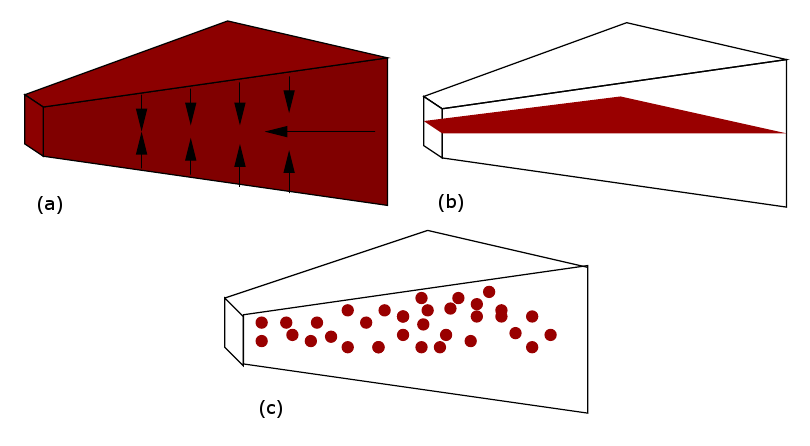
\includegraphics[width=0.9\textwidth]{figures/sedymentacja.png}
   \caption{Ilustracja mechanizmu Goldreicha-Warda. Połączenie sedymentacji pyłu
      na płaszczyznę dysku oraz jego radialnego dryfu (a) może prowadzić do
      wytworzenia się cienkiej i~masywnej warstwy pyłu (b), która jest
      niestabilna grawitacyjnie. Fragmentacja pod wpływem samograwitacji może
      prowadzić do wytworzenia się planetezymali w~lokalnych zagęszczeniach pyłu
      (c). Obrazek pochodzi z~pracy~\cite{armitage}
   }
   \label{fig:GW}
\end{figure}

\par Aby zrozumieć pewne niedostatki powyższej hipotezy, należy
dokładnie przeanalizować procesy zachodzące podczas ewolucji gazowo-pyłowego
dysku okołogwiazdowego. Syntetyczne zestawienie najbardziej istotnych
mechanizmów zostało przedstawione w~dalszej części tego rozdziału.

\par W przypadku gazowych olbrzymów powstających w masywnych dyskach
protoplanetarnych, alternatywną teoria zakłada kolaps i~fragmentację
grawitacyjną całego gazowo-pyłowego dysku~\cite{Boss97}. O tym czy zaburzenia
w~gęstości materii w~dysku będą wzrastać nieograniczenie decyduje równowaga
pomiędzy destabilizującym wpływem samograwitacji, a stabilizującymi
właściwościami ciśnienia oraz rotacji.  Wartość graniczna dla stabilności
cienkiego, osiowo symetrycznego dysku została pierwszy raz wyprowadzona przez
Toomre'ego~\cite{T64}, jako:
%
\begin{equation}
   Q = \frac{c_s\kappa}{\pi G \Sigma}\sim 1,
   \label{eq:toomre}
\end{equation}
%
gdzie $c_s$ to prędkość dźwięku, $\kappa$ częstość epicykliczna, $\Sigma$
gęstość powierzchniowa gazu. Kryterium to z~powodzeniem jest stosowane do
globalnych, stratyfikowanych dysków podlegających nieosiowo symetrycznym
zaburzeniom, tzn. symulacje numeryczne wykazują fragmentację takich dysków dla
$Q\sim 1$~\cite{NBAA98}. W ogólnym przypadku niestabilności grawitacyjnej dysku
kryterium stabilności jest zależne od azymutalnej liczby falowej
$m$~\cite{BT87}. Parameter Toomre'go~\mref{eq:toomre} jest wyprowadzony dla
$m=0$. Jak pokazują symulacje numeryczne~\cite{Duris07} efekt ten zachodzi już
dla $Q\lesssim 1.7$, a więc zanim dysk stanie się na tyle chłodny i~masywny, aby
ulec fragmentacji. Fale spiralne wytwarzają dodatkowe momenty sił i fale
uderzeniowe, które odpowiadają za transport masy i~momentu pędu oraz
podgrzewanie gazu~\cite{YC85}, stabilizując dysk. Kryterium~\mref{eq:toomre} nie
uwzględnia również destabilizujących efektów promienistego (bądź konwektywnego)
chłodzenia gazu~\cite{BMD06}. Dokładny przebieg niestabilności grawitacyjnej
w~realistycznych modelach dysków okołogwiazdowych jest ciągle
niejasny~\cite{MB11, LC11}. Niemniej jednak symulacje numeryczne sugerują, że w
masywnych dyskach niestabilność grawitacyjna jest w~stanie wytworzyć związane
obłoki materii o masach $\sim 1\div 10\Mjup$~\cite{BHM10, FR11}. Ich dalsza
ewolucja przebiega podobnie jak w~modelu akrecji jąder tj. pył sedymentuje na
centrum grawitacji tworząc skaliste jądro w~skalach czasowych od $10^3$ do
$10^6$ lat~\cite{HB11, GHB12}. Skalując parametry dysku względem typowych
wartości parametrów fizycznych obserwowanych w~dyskach protoplanetarnych,
parametr $Q$ można wyrazić jako:
%
\begin{equation}
   Q \sim 10^2 
   \left(\frac{T}{100\K}\right)^{0.5}
   \left(\frac{\Sigma}{10^3\g\cm^{-3}}\right)^{-1}
   \left(\frac{R}{1\AU}\right)^{-1.5}.
   \label{eq:Qemp}
\end{equation}
%
Z tego względu niestabilność grawitacyjna ma znaczenie tylko dla zewnętrznych
obszarów dysku protoplanetarnego. Co więcej, związane grawitacyjnie obłoki
podlegają silnemu oddziaływaniu pływowemu~\cite{VH12}, które może prowadzić do
ich rozerwania, a także gwałtownej migracji w~kierunku protogwiazdy~\cite{BMP11}.
\par Niestabilność grawitacyjna nie koniecznie wyklucza się z~modelem akrecji na
jądra, ponieważ może zachodzić już w~trakcie początkowych etapów formowania się
 układu protogwiazda -- dysk (pierwsze kilkaset tysięcy lat), w~przeciwieństwie do
 paru milionów lat w~przypadku akrecji na jądra. Niestabilność grawitacyjna
 również łatwiej tłumaczy powstawanie bardzo masywnych planet, które w~wypadku
 wiodącej teorii wymagają czasu porównywalnego z czasem życia dysku
 protoplanetarnego\cite{HBP}.


\begin{figure}[p]
\centering 
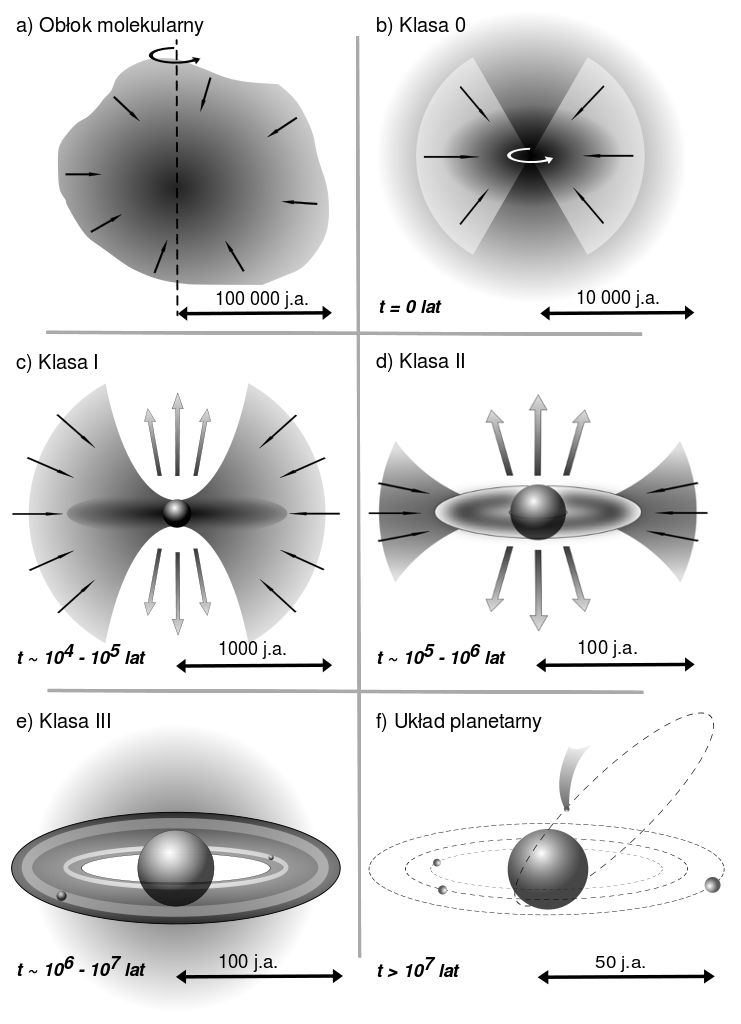
\includegraphics[width=0.9\textwidth]{figures/planetformation.png}
\caption{Ilustracja przedstawia kolejne fazy formowania się mało masywnej gwiazdy
   wraz z~systemem planetarnym: a) kolaps grawitacyjny gęstego obłoku; b)
   oddziaływanie centralnego pola grawitacyjnego oraz siły odśrodkowej powoduje
   opadanie materii i~formowanie się dysku; c) faza FU Orionis: silna akrecja w
   dysku oraz wypływ materii w~okolicach osi obrotu; d) faza T Tauri: zmniejsza
   się tempo akrecji $\sim 10^{-8}\Msun\rok^{-1}$ oraz wypływu materii,
   rozpoczyna się proces formowania planet; e) zanika składowa gazowa, planety
otwierają przerwy w~dysku, następuje również ich migracja; f) cały gaz oraz
mniejsze ciała zostają pochłonięte przez planety lub usunięte z~dysku, układ
planetarny przyjmuje ostateczny kształt. Obrazek zamieszczony dzięki uprzejmości
Joanny Drążkowskiej}

\label{fig:planet}
\end{figure}

\section{Ewolucja dysku protplanetarnego}
Planety formują się w gazowo--pyłowym dysku, który powstaje podczas kolapsu
obłoku protogwiazdowego. Pewne szczególne mechanizmy oraz globalna dynamika mogą
temu procesowi pomagać, bądź mu przeciwdziałać. Poniższe akapity pokrótce
opisują strukturę dysku protoplanetarnego oraz najważniejsze efekty dynamiczne
związane z~samym gazem, następnie przechodząc do ich wpływu na dynamikę
i~ewolucję pyłu. Pozwoli to wskazać problemy z~jakimi boryka się model ,,akrecji
na jądra'' i~naturalnie przejść do celu tej rozprawy.

\subsection{Struktura dysku protoplanetarnego}
W trackie kolapsu grawitacyjnego obłoku moment pędu jest zachowany. Gdy obłok
rotuje materia nie opada bezpośrednio na obiekt centralny, lecz formuje dysk
w~płaszczyźnie prostopadłej do wektora całkowitego momentu pędu. Aby określić
przybliżone warunki fizyczne w~formującym się dysku możemy posłużyć się
równaniami hydrodynamiki:
%
\begin{gather}
   \partial_t \rho_g + \nabla\cdot\left(\rho_g\mathbf{u}\right) = 0,
   \label{eq:hd1}\\
\partial_t \mathbf{u} + \left(\mathbf{u}\cdot\nabla\right)\mathbf{u} = 
-\nabla\Phi + -\frac{1}{\rho_g} \nabla P, \label{eq:hd2}
\end{gather}
%
gdzie $\rho_g$ jest gęstością gazu, $P$ ciśnieniem, 
związanych z~tarciem, a $\Phi$ potencjałem grawitacyjnym. Jeżeli ponadto
założymy, że dysk jest izotermiczny to
\begin{equation}
   P = n k_{\textrm{B}} T = \frac{\rho k_{\textrm{B}} T}{m_{\textrm{H}}} = \rho
   c_s^2 
\end{equation}
gdzie $c_s$ jest izotermiczną prędkością dźwięku. To implikuje, że gradient
ciśnienia można wyrazić przez:
\begin{equation}
   -\frac{1}{\rho_g}\nabla P = -c_s^2\nabla\ln\rho_g,
\end{equation}
%Przy założeniu stacjonarności równanie~\mref{eq:hd2} 
%
Gdy dysk znajduję się w~równowadze hydrostatycznej w~kierunku $z$ to wertykalne
przyspieszenie grawitacyjne:
%
\begin{equation}
   \partial_z \Phi = g_z = \frac{GM_\star}{r^2}\frac{z}{r} = \Omega^2 z,
\end{equation} 
%
gdzie $M_\star$ to masa gwiazdy macierzystej, $\Omega$ orbitalna częstość
keplerowska, $G$ stała grawitacji Newtona, jest równoważone przez gradient
ciśnienia gazu $\partial_z P / \rho_g$.
Łącząc powyższe założenia otrzymujemy rozkład gęstości gazu:
%
\begin{equation} \label{eq:zeq}
   \rho_g(z) = \frac{\Sigma_G}{H\sqrt{2\pi}} \exp \left[
   \frac{1}{2}\left(\frac{z}{H}\right)^2 \right],
\end{equation}
%
gdzie $\Sigma_g = \int \rho_g(z) dz$ jest gęstością powierzchniową, a
$H=\frac{c_s}{\Omega}$ to charakterystyczna skala grubości dysku.
%
%\par Zakładając w~pierwszym przybliżeniu że dysk jest optycznie gruby, t.j.
%absorbuję całkowicie promieniowanie pochodzące od gwiazdy i~następnie reemituje
%je jako ciało doskonale czarne, można pokazać~\cite{armitage07} że $T \propto
%r^{-3/4}$ i~co za tym idzie $c_s \propto r^{-3/8}$. Dokładniejsze szacunki,
%które lepiej oddają obserwowane dystrucje spektralne energii, można znaleźć w
%pracach~\cite{KenyonHART87, ChaingGold97} {\bf patrz armitage}.
%{\bf Tu raczej trzeba przedstawić tę wersję z~której wynika $T \propto
%r^{-1/2}$}
%
\par W~modelu stacjonarnym warunek równowagi sił radialnych można zapisać
równaniem:
%
\begin{equation}\label{eq:radial_balance}
\frac{u_\phi^2}{r} = \frac{GM_\star}{r^2} +
  \frac{1}{\rho_g}\frac{\textrm{d}P}{\textrm{dr}},
\end{equation}
gdzie $u_\phi^2$ jest prędkością orbitalną gazu.  Kolejne wyrazy
równania~\mref{eq:radial_balance} reprezentują: siłę odśrodkową, siłę
grawitacji, gradient ciśnienia. Wpływ tego ostatniego na globalny rozkład
prędkościjest rzędu $O(H/r)^2$. Dlatego dla cienkich dysków $(H/r \ll 1)$
z~dobrym przybliżeniem można przyjąć, że właściwy moment pędu gazu jest równy
momentowi pędu odpowiadającemu ruchowi keplerowskiemu. Z równania
\mref{eq:radial_balance} wynika zatem, że moment pędu jest monotonicznie rosnącą
funkcją promienia:
%
\begin{equation}\label{eq:angmom}
l = r^2\Omega = \sqrt{GM_\star r}.
\end{equation}
%
Aby materiał z~dysku mógł być akreowany przez gwiazdę macierzystą, w~układzie
musi działać mechanizm powodujący utratę, bądź chociaż redystrybucję momentu
pędu.

\subsection{Transport momentu pędu}
$\ldots$
Obserwacje 
Z obserwacji jasno wynika~\citep{MME04}, że dyski protoplanetarne nie są
obiektami stacjonarnymi. 

Co więcej, obiekty klasy I posiadają wysokie tempa
akrecji $\sim 10^{-5}\Msun\yr^{-1}$. Aby był możliwy radialny przepływ materii
w~kierunku gwiazdy macierzystej, potrzebny jest mechanizm transportu momentu
pędu. W~tym celu trzeba założyć, że ośrodek jest lepki. Zatem należy zastosować
równania Naviera--Stokesa, w których transport momentu pędu jest konsekwencją
siły lepkiej w różniczkowo rotującym dysku (ostatni wyraz po prawej stronie
równania~\mref{eq:ns2}):

\begin{gather}
   \partial_t \rho_g + \nabla\cdot\left(\rho_g\mathbf{u}\right) = 0,
   \label{eq:ns1}\\
\partial_t \mathbf{u} + \left(\mathbf{u}\cdot\nabla\right)\mathbf{u} = 
-\nabla\Phi -\frac{1}{\rho_g} \nabla P + \frac{1}{\rho_g} \nabla \cdot \Pi.
\label{eq:ns2}
\end{gather}
%
Jeżeli dodatkowo założymy, że mamy do czynienia z~płynem newtonowskim, tensor
naprężeń można zredukować do postaci $\Pi = (\rho_g \nu)\nabla\cdot\mathbf{u}$,
gdzie $\nu$ jest lepkością kinematyczną. Całkując układ
równań~\mref{eq:ns1}-\mref{eq:ns2} w~kierunku wertykalnym i~dokonując prostych
przekształceń można otrzymać
\begin{equation}\label{eq:sigma}
   \partial_t \Sigma_g =
   \frac{3}{R}\partial_R\left(\frac{1}{R\Omega}\partial_R\left(R^2\Sigma_g \nu
         \Omega\right)\right).
\end{equation}
Rozwiązaniem stacjonarnym równania~\mref{eq:sigma} jest warunek $\Sigma_g\nu =
\textrm{const}$, co przekłada się na tempo akrecji $\dot{M} = 3\pi\Sigma_g\nu$.
Z powyższego warunku wynika, że lepkość jest własnością ośrodka odpowiedzialną
za akrecję dyskową. Problemem pozostaje wskazanie mechanizmu fizycznego, który
daje przyczynek do lepkości.
\par Podstawowa lepkość, tj. lepkość molekularna $\nu_{\textrm{m}} \sim c_s
\lambda$, gdzie $\lambda = 1 / n\sigma$ to średnia droga swobodna molekuł gazu,
zaś $n$ to koncentracja molekuł gazu, a $\sigma$ ich przekrój czynny, dla
typowych wartości gęstości i~temperatury dysków protoplanetarnych wynosi
$\nu_{\textrm{m}}\sim10^5\cm^2\s^{-1}$~\cite{armitage}. Przekłada się to na
tempo akrecji na poziomie $\dot{M}\sim 10^{-17}\Msun\rok^{-1}$. 
Charakterystyczna skala czasowa takiego procesu $\tau \simeq R^2 /
\nu_{\textrm{m}}$ wynosiłaby $10^{13}\yr$. Z tego względu lepkość molekularną można
całkowicie zaniedbać w~dalszych rozważaniach.
\par W~słynnej pracy Shakura i~Sunyaev~\citep{SS73} zaproponowali, że turbulencja
w dysku może dawać znaczący przyczynek do lepkości, znacząco przeyższający
lepkość molekularną. Dla izotropowej turbulencji, maksymalna skala wirów w~dysku
powinna być proporcjonalna do charakterystycznej skali grubości dysku $H$, zaś
maksymalna prędkość ruchu turbulentnych nie powinna przekraczać prędkości
dźwięku, ponieważ fale uderzeniowe bardzo szybko dyssypują energię kinetyczną.
Shakura i~Sunyaev zaproponowali parametryzację lepkości turbulentnej:

\begin{equation}\label{eq:alpha}
\nu = \alpha c_s H,
\end{equation}
%
gdzie $\alpha$ jest bezwymiarowym parametrem określającym wydajność
turbulencji w~transporcie momentu pędu. Aby wyjaśnić obserwowane tempo akrecji
dla gwiazd \emph{T Tauri}, parametr $\alpha$ powinien być rzędu $10^{-2}$.
Problemem pozostaje wyjaśnienie mechanizmu powstawania turbulencji w~dysku. Z
kryterium Rayleigha~\cite{C61}:
%
\begin{equation}
   \frac{\mathrm{d}}{\mathrm{d}r} j =
   \frac{\mathrm{d}}{\mathrm{d}r}\left(r^2\Omega\right) > 0,
\end{equation}
%
wynika, że hydrodynamiczny dysk keplerowski jest liniowo stabilny. Sytuacja
diametralnie się zmienia jeżeli uwzględnimy obecność w~układzie 
słabego pola magnetycznego. Balbus i~Hawley~\citep{BH91} pokazali, że przepływ
magnetohydrodynamiczny jest stabilny liniowo wtedy i~tylko wtedy, gdy:
%
\begin{equation}\label{eq:mri}
   \frac{\mathrm{d}}{\mathrm{d}r}\left(\Omega^2\right) > 0.
\end{equation}
%
Warunek \mref{eq:mri} \emph{nie jest} spełniony dla dysków keplerowskich. W
rezultacie nawet szczątkowe pole magnetyczne, jest w~stanie wzmocnić wykładniczo
zaburzenia prędkości oraz pola magnetycznego w~gazie w~czasie kilku okresów
orbitalnych, powodując silną
turbulencję. Proces ten określany jest mianem niestabilności magnetorotacyjnej
(MRI). Co więcej, zarówno symulacje lokalne~\cite{DSP10}, jak
i globalne~\cite{FD11} szacują parametr lepkości $\alpha$ dla dysku, w którym
turbulencja została wzbudzona przez MRI na $\alpha\sim 10^{-2}$.
\par Należy zauważyć, że niestabilność magnetorotacyjna wymaga choćby
szczątkowej jonizacji gazu. 

$\ldots$
Jeżeli założymy że źródłem jonizacji jest wysoko energetyczne
promieniowanie pochodzące od gwiazdy macierzystej i~weźmiemy pod uwagę strukturę
pionową dysku~\mref{eq:zeq}, to dojdziemy do wniosku, iż od pewnej wysokości
$h_i$ materia w dysku jest efektywnie osłaniana przez warstwy gazu o $h > h_i$, gdzie
$h_i$ jest wysokością podstawy

zjonizowanego gazu. 
Obszar $h < h_i$ jest zatem \emph{martwą strefą}
w której niestabilność magnetorotacyjna nie występuje~\cite{DFT10} i nie może
być zatem źródłem turbulencji. 

\begin{figure}
   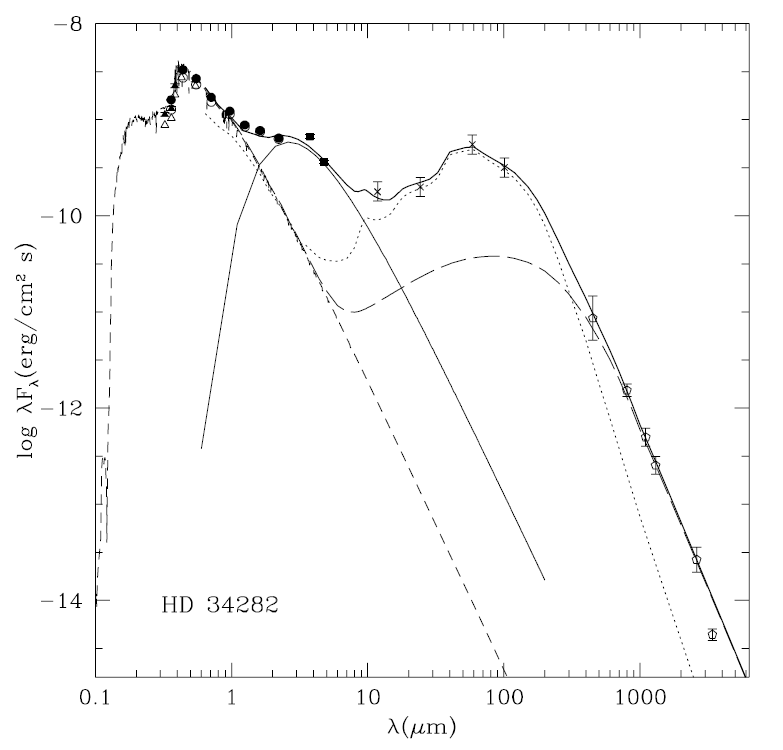
\includegraphics[width=0.9\textwidth]{figures/chap1_sed.png}
   \caption{Rozkład widma energii dla gwiazdy HD 34282~\cite{MME4}. Symbole oznaczają
      obserwacje różnymi metodami dla odpowiednich długości fali. Do obserwacji
      dopasowano następujące modele: linia przerywana model widma gwiazdowego
      dla obiektu typu A3V $(T\sim 8600\K)$, cienka ciągła
      linia model ciała doskonale czarnego dla $T=1400\K$,
      linia kropkowana reprezentuje model dysku o nachyleniu $i=56^o$, tempie
      akrecji $\dot{M} = 8.2\times10^{-9}\thinspace\Msun\yr^{-1}$
      rozciągającym się od $0.31\AU$ do $705\AU$.
   Obrazek pochodzi z~pracy~\cite{MME04}}
   \label{fig:sed}
\end{figure}

\subsection{Oddziaływanie pomiędzy gazem, a pyłem}
Oddziaływanie pomiędzy pyłem a gazem odbywa się poprzez tarcie aerodynamiczne.
Charakterystyczną skalę czasową tego procesu można wyrazić jako~\cite{W73}:
%
\begin{equation}
   \tau_f = \frac{mv_\textrm{pg}}{F_\textrm{D}},
\end{equation}
%
gdzie $m$ i~$v_{\textrm{pg}}\equiv|\mathbf{u} - \mathbf{v}|$ to odpowiednio masa
i prędkość cząstek pyłu względem gazu, zaś $F_\textrm{D}$ to siła tarcia.
$\tau_f$ można interpretować jako czas potrzebny do wytracenia pędu cząstki pyłu
i zrównania jej prędkości z~gazem. Siła $F_\textrm{D}$ jest definiowana w~różny
sposób, w~zależności od rozmiaru ziaren pyłu. Dla cząstek pyłu o promieniu $a < 9
\lambda / 4$ siła tarcia wyraża się prawem Epsteina~\cite{W77}:
%
\begin{equation}
   F_\textrm{D} = \frac{4}{3}\pi a^2 \rho_\bullet \rho_G c_s v_\textrm{pg}, 
\end{equation}
%
gdzie $\rho_\bullet = 1.6\g\cm^{-3}$ jest gęstością materiału, z~którego
zbudowany jest pył. Dla ziaren pyłu o rozmiarach porównywalnych z~drogą swobodną
molekuł gazu, siła tarcia wyraża się poprzez prawo Stokesa~\cite{W77}:
\begin{equation}
  F_\textrm{D} = C_\textrm{D} \pi a^2 \rho \frac{v^2}{2},
\end{equation}
gdzie $v$ to prędkość gazu, zaś współczynnik $C_\textrm{D}$ jest zależny od
liczby Reynoldsa~\cite{W77}:
\begin{equation}
   \textrm{Re} = 2 a \rho \frac{v}{\eta}.
   \label{eq:Re}
\end{equation}
Parametr $\eta$ w równaniu \mref{eq:Re} jest lepkością gazu.
W~niniejszej pracy skupiono się
na obszarach dysków rozciągających się od relatywnie dużych promieni, tj.
$>2\AU$.  Biorąc pod uwagę, iż średnią drogę swobodną możemy wyrazić przez
$\lambda_g = 4.2\times 10^4\textrm{ cm} (10^{-14}\textrm{ g cm}^{-3}/\rho_g)
\approx (R/1 \textrm{AU})^{2.75}\cm$~\citep{W77,BT09}, gdzie $R$ jest odległością
radialną od centrum dysku, prawo Epsteina ma zastosowanie dla dominującej części
domeny obliczeniowej nawet dla największych symulowanych przez nas ziaren pyłu.
Skalę czasową tarcia można wyrazić wzorem:
%
\begin{equation} 
   \tau_f = \frac{\rho_\bullet a} {\rho_g \sqrt{c_s^2 +
      |\mathbf{u} - \mathbf{w}|^2 }} \label{eq:tauf} 
\end{equation}
%
Powodem różnicy prędkości pomiędzy pyłem a gazem może być wiele
procesów, przede wszystkim turbulencja obecna w~gazie, ale także radialny dryf
pyłu (o którym będzie mowa w~dalszej części tego rozdziału) oraz ruchy
Browna. Te ostatnie bardzo silnie zależą od rozmiaru cząstek, tj.
makroskopowe cząstki pyłu praktycznie nie odczuwają ich wpływu, nie są zaś
zależne od gęstości gazu. Ruchy Browna są niezwykle istotne dla rozpoczęcia
procesów koagulacji pyłu w~początkowej fazie formacji
protoplanet~\citep{DD05}, ponieważ skutkują dość znacznym prędkościom względnym
dla najmniejszych ziaren pyłu, które są najsilniej związane z~gazem. Turbulencja
i radialny dryf natomiast tym silniej wpływają na dynamikę, im większa jest
gęstość gazu. Ich znaczenie jest większe dla cząstek o rozmiarach pośrednich, które
są słabie sprzężone z chaotycznymi ruchami gazu.

\subsection{Radialny dryf pyłu}
Jedno z przybliżeń stosowanych w opisie dysków gazowo-pyłowych opiera się na
załóżeniu, że pył w~dysku protoplanetarnym można traktować jako bezciśnieniowy płyn. 
Jako że gęstość materii w~dysku zgodnie z założeniami jest malejącą funkcją
promienia, to dla izotermicznego gazu gradient ciśnienia jest ujemny dla całej
rozciągłości dysku. W~rezultacie radialna składowa siły grawitacyjnej dla gazu
jest pomniejszona o gradient ciśnienia. Równanie równowagi sił radialnych:
%
\begin{equation}
   R\Omega_g^2 = \partial_R P / \rho_G + R\Omega_K^2
\end{equation}
%
implikuje, że prędkość orbitalna dla gazu jest nieznacznie mniejsza niż prędkość
keplerowska. Niedobór prędkości rotacji gazu $\delta v = \eta v_\textrm{K}$
względem prędkości orbitalnej opisanej prawem Keplera można określić się jako
bezwymiarowym parametrem~\cite{N86} wyrażonym jako:
%
\begin{equation}
   \label{eq:eta}
   \eta = \frac{\partial_R P}{2\rho_\textrm{G} R \Omega^2} = \frac{1}{2}
   \frac{c_s^2}{v_\textrm{K}^2} \partial_{\ln r} \ln \rho_{\textrm{G}} \approx
   \frac{c_s^2}{v_\textrm{K}^2}.
\end{equation}
%
Dla typowych wartość parametrów, na promieniu $1\AU$, przy $v_\textrm{K}\approx
30\km\s^{-1}$ i~$\eta \approx 10^{-3}$ różnica w~prędkości orbitalnej między
gazem a pyłem wynosi $\Delta v \approx 33\m\s^{-1}$.  W~rezultacie cząstki pyłu
odczuwają permanentny ,,wiatr w~oczy'' skierowany przeciwnie do kierunku ruchu
orbitalnego i~na skutek tarcia trąca swój moment pędu. Efektywność tego procesu
silnie zależy od rozmiaru ziaren pyłu. Drobne cząstki są silnie związane z~gazem
i przez to porusząją się z prędkością bliską prędkości gazu. W rezultacie efekt
oporu aerodynamicznego jest zaniedbywalny. Podobnie dla dużych i~masywnych
obiektów ze względu na ich bezwładność. Najsilniejsza utrata momentu pędu
następuje dla ziaren pyłu spełniających relację $\Omega \tau_f \sim 1$, co
odpowiada cząstkom pyłu o rozmiarach $1\m$ na orbicie o promieniu $1\AU$, bądź
$10\cm$ w~zewnętrznych obszarach dysku.

\begin{figure}
   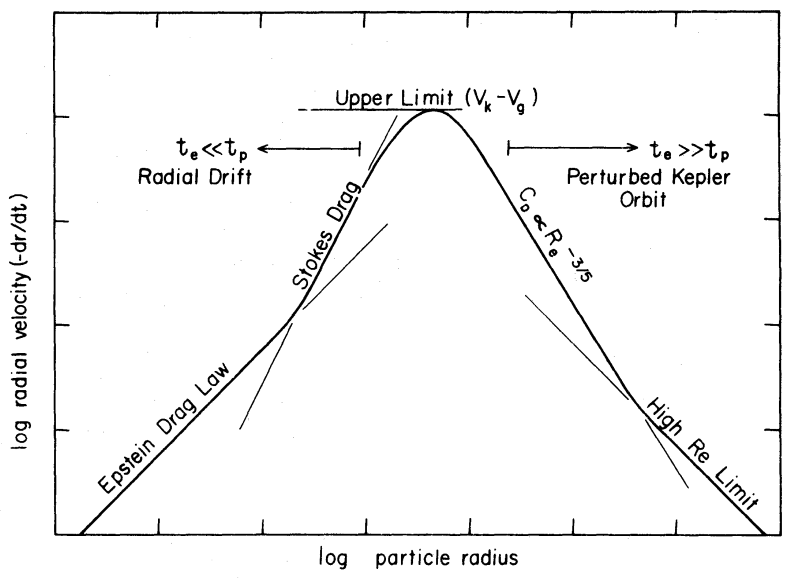
\includegraphics[width=0.9\textwidth]{figures/chap1_drift.png}
   \caption{Schematyczny rysunek zależności pomiędzy rozmiarem ziaren pyłu, a
   maksymalną prędkością radialnego dryfu. Obrazek pochodzi z
   pracy~\cite{W77}}
   \label{fig:chap1_drift}
\end{figure}

Ziarna te są w~stanie osiągać prędkości radialne rzędu
$10^2\div10^3\cm\s^{-1}$~\cite{W77}, co przekłada się na ucieczkę tych cząstek w
kierunku centralnej gwiazdy w~skali czasowej rzędu setek lat!  Kolejną
konsekwencją zależności radialnego dryfu od rozmiaru cząstek jest zróżnicowanie
ich prędkości względem siebie. Cząstki pyłu sklejają się dzięki oddziaływaniom
międzycząsteczkowym, które są szczególnie wydajne w~przypadku małych cząstek
i~dużego ich zagęszczenia. Wraz ze wzrostem cząstek proces zlepiania zachodzi
coraz wolniej.  Siły elektrostatyczne faworyzują małe cząstki, które mają większy stosunek
powierzchni do masy. Przy odpowiednio niskiej prędkości względnej kolizje
prowadzą do tworzenia coraz to większych aglomeratów cząstek~\citep{BW08}, ale
dla dużych różnic w prędkościach najbardziej prawdopodobnym rezultatem zderzenia
jest fragmentacja bądź odbicie~\citep{Z10}. 

\par Nie dość, że czas w którym ziarna pyłu o rozmiarach $0.1 \div 10\m$ mogły
by rosnąć jest niezmiernie krótki, to nie jesteśmy w~stanie wskazać żadnego
mechanizmu powodującego dalszy wzrost rozmiarów pyłu. Problem ten nosi nazwę
\emph{metrowej bariery wzrostu} i~jest najważniejszą niewyjaśnioną kwestię
obecnego paradygmatu formacji planet. 

\par W~ogólności dryf radialny przemieszcza pył w~kierunku maksimum ciśnienia w
gazie. Dla modelu dysku, w którym rozkład gęstości jest opisany funkcją
wykładniczą jest to tożsame z~centrum grawitacji. Należy jednak pamiętać, że
turbulentny ośrodek może wytwarzać lokalne, przejściowe maksima w~ciśnieniu
gazu, dla których gradient będzie dużo większy niż gradient globalny. Z tego
względu obszary o podwyższonym ciśnieniu będą działać jako swoiste pułapki na
pył, przejściowo zwiększając jego gęstość.  Cuzzi, Hogan i~Shariff~\citep{CHS08}
postulują, iż przejściowe zagęszczenia pyłu na skutek ruchów turbulentnych są
wyzwalaczem dla dalszych procesów formowania się planetezymali.
%
\begin{figure}
   \centering
   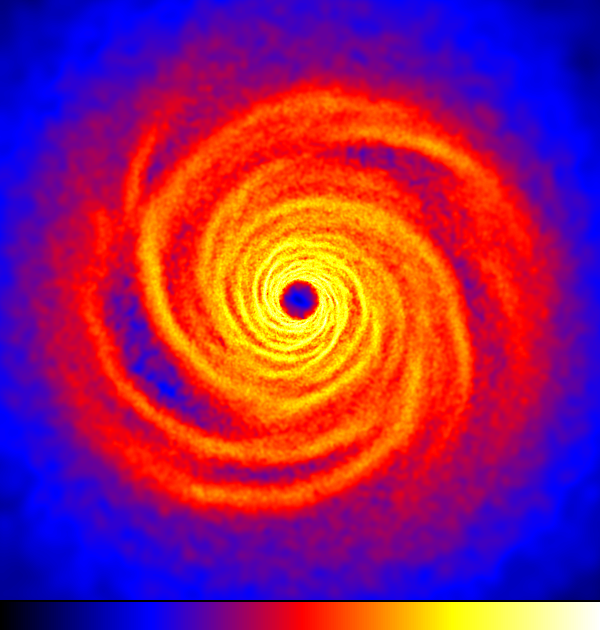
\includegraphics[width=0.46\textwidth]{figures/chap1_gasdisk.png}
   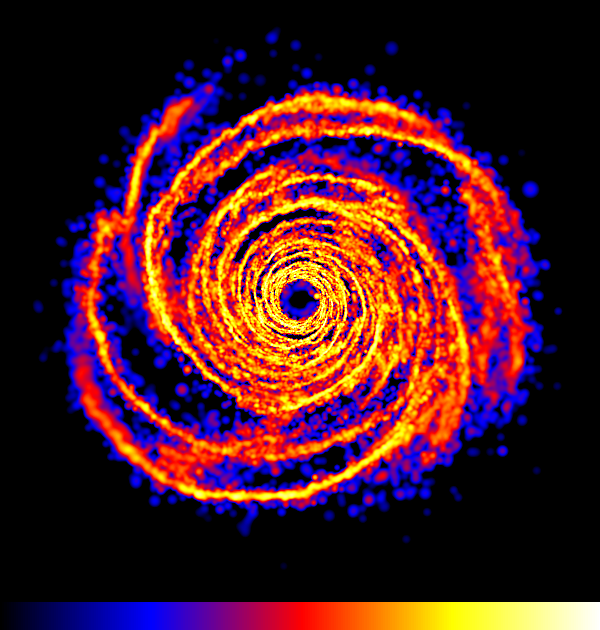
\includegraphics[width=0.46\textwidth]{figures/chap1_dustdisk.png}
   \caption{Symulacja dwuskładnikowego, izotermicznego dysku
      pro\-to\-pla\-ne\-tar\-ne\-go.
      Lewy panel przedstawia rozkład ciśnienia gazu, prawy zaś rozkład gęstości
      gazu. Wy\-raź\-nie widać jak pył jest pułapkowany w~lokalnych maksimach
      ciśnienia. Obrazek za\-po\-ży\-czo\-ny~z pracy~\cite{RLP2006}}
   \label{fig:chap1_trap}
\end{figure}

\subsection{Sedymentacja i~niestabilność Kelvina-Helmholtza (KHI)}
W~dotychczasowych rozważaniach pominęliśmy wpływ pionowej składowej siły
grawitacji pochodzącej od gwiazdy macierzystej na dynamikę ziaren pyłu. O ile
gaz zostaje ściśnięty przez grawitację do momentu osiągnięcia równowagi
hydrostatycznej z gradientem ciśnienia~\mref{eq:zeq}, o tyle opadaniu pyłu nie
przeciwdziała żaden proces fizyczny~\footnote{na chwilę pomińmy fakt, że gaz
jest ośrodkiem turbulentnym i~przez wzajemne sprzężenie wpływa na dynamikę
pyłu}. Sedymentacja mogłaby zatem prowadzić do wytworzenia się cienkiej i~bardzo
gęstej warstwy pyłu, która po przekroczeniu wartości krytycznej rozpadłaby się
pod własnym ciężarem~\citep{GW73}. Zauważmy jednak, że osiadanie pyłu prowadzi
do stopniowego zwiększenia stosunku gęstości pyłu do gazu w~płaszczyźnie dysku.
Ponadto, jak już było wspomniane w~poprzednim podrozdziale, pył porusza się na
wybranej orbicie z~prędkością keplerowską, natomiast gaz pod wpływem radialnego
gradientu ciśnienia z~prędkością podkeplerowską. Duża koncentracja pyłu
w~płaszczyźnie powoduje, że gaz jest efektywniej ,,pchany'' przez pył i~zaczyna
poruszać się szybciej niż warstwy gazu leżące poniżej i~powyżej płaszczyzny
rotacji dysku.  Prowadzi to do wytworzenia się pionowego gradientu prędkości
azymutalnej gazu.  Taka sytuacja powoduje wzbudzenie niestabilności
Kelvina-Helmholtza i~pojawienie się turbulencji w~gazie.  Na skutek wzajemnego
sprzężenia turbulentne ruchy gazu skutkują mieszaniem składnika pyłowego
i~hamowaniem sedymentacji~\cite{JHK06}. Niedawne badania pokazują że tylko
bardzo masywne dyski, o~metaliczności dużo większej niż słoneczna, są nie
wrażliwe na ten proces~\citep{L10}. Podobnie jak w~przypadku niestabilności
magnetorotacyjnej turbulentne ruchy gazu skutkują analogicznymi ruchami pyłu,
jednakże i~w~tym wypadku ustala się pewien stan równowagi dynamicznej między
sedymentacją pyłu, a turbulencją~\cite{JHK06}. 

\subsection{Niestabilność strumieniowa}
Pomimo działania turbulencji wywołanej poprzez szereg opisywanych wcześniej
niestabilności płynowych, w~dysku protoplanetarnym może uformować się warstwa
pyłu o skończonej grubości, dużo mniejszej niż grubość dysku gazowego. Pył ten
jest jednak zbyt rzadki, aby wzbudziła się w~nim niestabilność
grawitacyjna~\cite{JHK06} {\bf jeszcze praca AJ o MRI}.
\par Pomimo tych niesprzyjających warunków istnieje proces który dominuje
ewolucję pyłu w~momencie w~którym stosunek geśtości pyłu do gęstości
gazu zbliża się do jedności. Tym mechanizmem jest {\it niestabilność
strumieniowa} po raz pierwszy przedstawiona w~pracy~\cite{YG05}. Wraz ze
wzrostem gęstości pyłu spowodowanego jego dryfem w~kierunku najbliższego
maksimum ciśnienia gazu, wzrasta wypadkowa siła z~jaką pył oddziałuje na gaz.
Prowadzi to zwiększenia prędkości gazu i~wzrostu ciśnienia na skutek zagarniania
obszarów gazów poruszających się wolniej. Zwiększa to maksimum ciśnienia w~gazie
i przyspiesza dryft pyłu z~otaczających go obszarów. W~przypadku braku działania
dodatkowych sił, gradient ciśnienia skierowany na zewnątrz gęstniejącego obszaru
powodowałby jego szybkie rozmycie, ale w~wypadku rotującego dysku połączenie
ciągłego dryfu pyłu i~siły Coriolisa prowadzi do wytworzenia się równowagi
geostroficznej~\cite{JBL11}. Nasycenie gęstości pyłu następuje w~momencie gdy
masa porcji pyłu jest w~stanie wyrwać się z~lokalnego maksimum gazu.  Nawet
zaniedbując efekt samograwitacji w~trakcie ewolucji niestabilności strumieniowej
lokalna gęstość pyłu może zwiększyć się tysiąckrotnie~\cite{JY07}, co może
prowadzić do wytworzenia się grawitacyjnie związanych obiektów~\cite{J07}.
Niedawne badania niestabilności strumieniowej skupiały się na różnych aspektach
fizycznych które mają wpływ na jej rozwój t.j.: uwzględnienie szerokiego
spektrum rozmiaru cząstek pyłu~\cite{BS10a}, wpływ globalnego gradientu
ciśnienia w~dysku okołogwiazdowym~\cite{BS10b}, stratyfikacja dysku~\cite{T12}.
Niemniej jednak wszystkie publikacje były ograniczone do lokalnego
przybliżenia dysku.

\section{Cel i plan pracy}
Głównym celem pracy jest zbadanie niestabilności strumieniowej w~
realistycznym przybliżeniu radialnie rozciągłego dysku.

Celem badań jest oszacowanie i~opis wpływu niestabilności strumieniowej na
proces generowania lokalnego wzrostu stosunku gęstości pyłu do gazu w~globalnym
dysku pyłowo-gazowym. Pył jako ważny składnik dysku okołogwiazdowego można
opisywać w~przybliżeniu płynowym (funkcja już zaimplementowana w~kodzie PIERNIK
patrz (Hanasz, et al. 2009b) lub w~przybliżeniu punktów materialnych. Obecnie w
literaturze naukowej dominuje druga  metoda, ważne jest więc jakościowa
i~ilościowa weryfikacja własności niestabilności strumieniowej w przybliżeniu
płynowym.


%%%%%%%%%%%%%%%%%%%%%%%%%%%%%%%%%%%%%%%%%%%%%%%%%%%%%%%%%%%%%%%%%%%%%%%%%%%%%%%%
% vim: tw=80 ts=3: 
